\documentclass[10pt]{article}

\usepackage[a4paper,margin=0.78in]{geometry}
\usepackage{amsmath,amssymb,amsthm,mathtools,bm}
\usepackage{booktabs,tabularx,longtable,microtype,enumitem,multicol,float}
\usepackage{xcolor,tikz}
\usetikzlibrary{arrows.meta,positioning,fit,calc}
\usepackage[colorlinks=true,linkcolor=blue!50!black,
  citecolor=blue!50!black,urlcolor=blue!50!black]{hyperref}

\newtheorem{theorem}{Theorem}
\newtheorem{corollary}[theorem]{Corollary}
\newtheorem{proposition}[theorem]{Proposition}
\theoremstyle{definition}
\newtheorem{definition}[theorem]{Definition}

\newcommand{\R}{\mathbb R}
\newcommand{\C}{\mathbb C}
\newcommand{\N}{\mathbb N}
\newcommand{\Z}{\mathbb Z}
\newcommand{\Q}{\mathbb Q}
\newcommand{\T}{\mathbb T}
\newcommand{\ee}{\mathrm e}
\newcommand{\ii}{\mathrm i}
\newcommand{\rank}{\operatorname{rank}}
\newcommand{\Rel}{\mathcal L}
\newcommand{\Hull}{\mathcal T}
\newcommand{\Carrier}{\mathcal C}
\newcommand{\Hwater}{\mathcal H}
\newcommand{\Fid}{\mathcal F}
\newcommand{\sinc}{\operatorname{sinc}}

\title{\textbf{Persistent phase geometry of quantum recurrence}\\
\large Four structural laws for loss, spectral constraints, observability, and finite-horizon inference}
\author{Michael Haufschild}
\date{5 August 2026}

\begin{document}
\maketitle

\begin{abstract}
Quantum recurrence is usually divided into separate questions about existence,
waiting time, observability, dissipation and prediction.  We prove that these
are shadows of one object: the persistent projective phase geometry selected
by the evolution and the observer.  It consists of a persistent spectral
carrier, the kernel of its balanced energy-detuning map, and an
observer-weighted metric on the resulting compact phase hull.

Four laws follow.  First, dissipation selects the carrier: for every finite
contraction, peripheral spectral mass is the exact asymptotic return-amplitude
ceiling, while arbitrary stationary spectra obey a point-spectrum and
collision-hierarchy law.  Second, constraints and temporal directions are
conserved.  On a finite $D$-level carrier,
\[
  \tau+\rho=D-1,
\]
and the completed future is exactly the annihilator of the balanced relation
lattice.  Interactions remove relations and convert them one-for-one into
phase directions.  This mechanism persists under geometric locality: for
every $n,q\ge2$, almost every traceless static Hamiltonian with arbitrary
onsite and nearest-neighbour terms on an open $q$-level chain has
$\rho=0$ and $\tau=q^n-1$.  The maximal set is dense and residual as well
as full measure.  Its strict projective-return frequency is exactly
\[
 \left[\frac{2\arcsin(\varepsilon/2)}{\pi}\right]^{q^n-1},
\]
and time zero is its only exact projective return.  At every fixed strict
tolerance this completed-time density tends to zero with exact rate
$-q^{-n}\log d_n\to-\log[2\arcsin(\varepsilon/2)/\pi]$; equivalently it
decays doubly exponentially in chain length.

Third, a single reverse-water functional controls both intrinsic return-target
information and the least worst-spectrum recurrence deadline, with explicit
finite errors; a coherence graph gives the exact phase capacity visible to
any finite observer.  Fourth, finite-horizon records do not stably determine
the completed geometry.  For any finite number of energy moments, any strict observation
window and any target time, one fixed state and projector admit an isospectral
family of nonnegative nearest-neighbour Hamiltonians whose earlier return
records agree arbitrarily well while the later return probability fills
$[0,1]$.  The construction lifts to all free-fermion sectors, has a sharp
spectral-support threshold, and forces minimax forecast error $1/2$.
Together the laws cover closed and contractive finite dynamics, countable
pure-point systems, arbitrary stationary spectral measures, local spin
realizations and exact inference limits without random-matrix or
nonresonance assumptions.
\end{abstract}

\noindent\textbf{One-sentence summary.}
Loss selects which phases survive, interactions remove their exact
constraints, observers decide their metric cost, and finite-horizon records
do not stably determine the completed phase geometry.

\section{One object behind four recurrence problems}

The quantum recurrence theorem guarantees approximate returns for finite
closed systems \cite{BocchieriLoinger1957}.  Recent work bounds recurrence
times for arbitrary and random spectra \cite{KotowskiOszmaniec2026,
GuptaShort2026}, identifies exact arithmetic Floquet periods
\cite{AnandEtAl2026}, reports isolated many-body recurrences
\cite{RauerEtAl2018}, and proposes coupled-multiqubit recurrence tests
\cite{KarimiEtAl2026}.  A unified treatment must answer four questions:
\begin{equation}
 \boxed{\text{What survives?}\quad\text{What constrains it?}\quad
 \text{What does an observer resolve?}\quad\text{What can a record predict?}}
 \label{eq:fourquestions}
\end{equation}

We show that all four questions act on the same ordered data,
\begin{equation}
 \text{persistent carrier}
 \longrightarrow
 \text{relation kernel / phase hull}
 \longrightarrow
 \text{observer metric}
 \longrightarrow
 \text{finite-horizon record}.
 \label{eq:pipeline}
\end{equation}
This ordering matters.  Dissipation can delete phase coordinates.  An
interaction can retain the carrier but remove exact relations.  An observer
can be blind to directions present in the full hull.  Finally, a scalar
return record known to any prescribed positive uniform accuracy on a strict
finite interval need not stably identify the geometry that determines a
later return.

Abstract torus dynamics alone does not show whether strict spatial locality
can realize the full projective phase rank of an exponentially large Hilbert
space.  Existing no-resonance and recurrence results either assume the
relevant arithmetic condition, establish only finite-order gap
nondegeneracy, or use unrestricted or random spectra
\cite{Huang2021,RiddellBertini2024,CamposVenutiOdavicHamma2026}.  Here a
static, finite-range, bounded-degree family is shown to eliminate every
nontrivial balanced relation generically.

A distinct question is whether finite observations identify the phase
geometry that controls later recurrence.  General quantum extrapolation
results exhibit broad ``fog-bank'' phenomena
\cite{ManosWeilenmannNavascues2025}.  The theorem proved here isolates a
fixed-protocol boundary with a common spectrum, local nearest-neighbour
generators, arbitrary finite moment agreement, arbitrarily accurate uniform
continuous-window agreement, and every exact later return probability.

\begin{figure}[t]
\centering
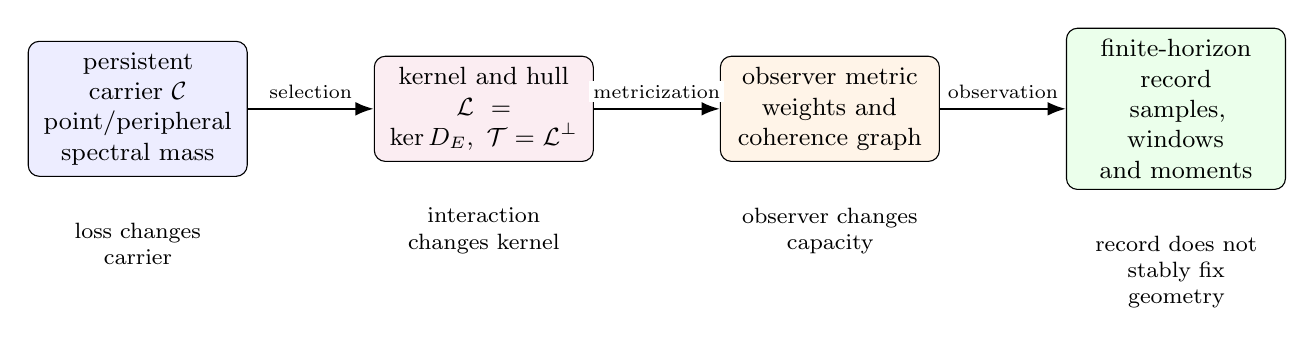
\begin{tikzpicture}[
  font=\small,>=Latex,
  box/.style={draw,rounded corners,align=center,text width=2.50cm,
    minimum height=1.25cm,inner sep=4pt},
  arr/.style={->,thick},
  arrowlabel/.style={font=\scriptsize,fill=white,inner sep=1.5pt},
  note/.style={align=center,font=\footnotesize,text width=2.50cm}
]
\node[box,fill=blue!7] (c) {persistent carrier $\Carrier$\\
  point/peripheral spectral mass};
\node[box,fill=purple!7,right=1.60cm of c] (k)
  {kernel and hull\\$\Rel=\ker D_E,\ \Hull=\Rel^\perp$};
\node[box,fill=orange!9,right=1.60cm of k] (m)
  {observer metric\\weights and coherence graph};
\node[box,fill=green!8,right=1.60cm of m] (r)
  {finite-horizon record\\samples, windows\\and moments};
\draw[arr] (c)--node[above=2pt,arrowlabel]{selection}(k);
\draw[arr] (k)--node[above=2pt,arrowlabel]{metricization}(m);
\draw[arr] (m)--node[above=2pt,arrowlabel]{observation}(r);
\node[note,below=0.46cm of c] {loss changes carrier};
\node[note,below=0.46cm of k] {interaction changes kernel};
\node[note,below=0.46cm of m] {observer changes capacity};
\node[note,below=0.46cm of r] {record does not\\stably fix geometry};
\end{tikzpicture}
\caption{\textbf{Persistent phase geometry.}  Four apparently separate
recurrence problems are successive transformations or restrictions of one
object.}
\label{fig:geometry}
\end{figure}

\section{Persistent phase geometry}

Consider first a finite pure-point packet with distinct occupied energies
$E=(E_j)_{j\in\Carrier}$, positive weights $w_j$, and
$\sum_jw_j=1$.  Global phase is physically invisible, so integer
characters must be balanced.  Define
\begin{align}
 P_{\Carrier}&=\left\{k\in\Z^{\Carrier}:\sum_jk_j=0\right\},
 \label{eq:projectivecharacters}\\
 D_E(k)&=\sum_j k_jE_j,\qquad
 \Rel_E=\ker D_E,                                      \label{eq:detuning}\\
 \Hull_E&=\left\{z\in\T^{\Carrier}/\T:
             z^k=1\ \text{for all }k\in\Rel_E\right\}. \label{eq:hull}
\end{align}
The relation rank is $\rho(E)=\rank_{\Z}\Rel_E$.  The temporal rank is
\begin{equation}
 \tau(E)=\dim_{\Q}\operatorname{span}_{\Q}
       \{E_j-E_{j_0}:j\ne j_0\},                       \label{eq:tau}
\end{equation}
independent of the anchor $j_0$.  The orbit closure of
$t\mapsto(\ee^{-\ii t(E_j-E_{j_0})})_{j\ne j_0}$ is $\Hull_E$.
For a balanced character $k$, write $k=k^+-k^-$ with disjoint
nonnegative parts and define its height by
$h(k)=|k^+|_1=|k^-|_1$.  The order-$r$ fidelity replica is
$|\sum_jw_jz_j|^{2r}$.  Throughout,
$\sinc(u)=\sin(u)/u$ for $u\ne0$ and $\sinc(0)=1$.

The state supplies a metric through its fidelity defect
\begin{equation}
 d_w(z)=1-\left|\sum_jw_jz_j\right|.                    \label{eq:metric}
\end{equation}
More general observers replace $d_w$ by an exact phase-energy quadratic
form.  For nonunitary finite dynamics, the carrier is the semisimple
peripheral spectral packet.  For arbitrary stationary spectral measures it
is the pure-point component, with continuous parts contributing to the
collision law but not persistent coherent mass.  These definitions lead to
four laws.

\section{Law I: loss selects the persistent carrier}

Let $T$ be a contraction on a finite-dimensional complex Hilbert space and
let $x$ be an initial vector.  The peripheral eigenvalues
$|\lambda|=1$ are semisimple.  Writing $x_{\lambda}$ for the corresponding
spectral components, define
\begin{equation}
 M_{\rm per}(T,x)=\sum_{|\lambda|=1}\|x_{\lambda}\|^2. \label{eq:peripheral}
\end{equation}

\begin{theorem}[Persistent-carrier selection law]
\label{thm:carrier}
For every finite contraction $T$ and vector $x$,
\begin{equation}
 \langle x,T^nx\rangle
 =\sum_{|\lambda|=1}\lambda^n\|x_\lambda\|^2+r_n,
 \qquad r_n\longrightarrow0.                           \label{eq:persistentdecomp}
\end{equation}
The scalar $M_{\rm per}(T,x)$ is the exact asymptotic return-amplitude
ceiling: every target strictly below it is reached after every prescribed
delay, whereas every target strictly above it is eventually impossible.
When at least two persistent modes survive, a quantitative post-burn-in
deadline is supplied by the weighted phase clock of Law III.
\end{theorem}

Thus loss acts before arithmetic: it removes transient coordinates, and
recurrence takes place on the surviving torus.  The theorem includes unitary
dynamics as $M_{\rm per}=\|x\|^2$, finite convex mixtures of contractions,
and contractive transfer operators on finite operator spaces.

There is also an arbitrary-spectrum stationary law.  Let $\mu$ be a
probability measure on energies and
$A_\mu(t)=\int\ee^{\ii tE}\,d\mu(E)$.  Every continuous statistic of
$|A_\mu(t)|^2$ has a long-time mean.  For every replica order $r$, the
mean of $|A_\mu(t)|^{2r}$ converges to the zero-gap mass of the $r$-fold
convolution of the spectral difference measure.  In particular, stationary
mean fidelity is exactly the squared total mass of the atoms, with their
individual weights retained.  For atomless $\mu$, every fixed
positive-fidelity window has asymptotic density zero and the projective
observer phase dimension is continuum.  Conversely, every nonnegative
summable countable pure-point phase packet recurs below every positive
phase-energy resolution.  Exact unit-fidelity return occurs precisely when
the additive group generated by differences in the spectral support is
cyclic.  These statements distinguish
absence of persistent mass, approximate recurrence of summable point
spectra, and exact periodicity.

\section{Law II: constraints are converted into time}

\begin{theorem}[Kernel--quotient conservation]
\label{thm:kernel}
For every finite $D$-level carrier,
\begin{equation}
 0\longrightarrow\Rel_E\longrightarrow P_{\Carrier}
  \xrightarrow{D_E}\operatorname{span}_{\Q}\{E_j-E_{j_0}\}
  \longrightarrow0,
 \qquad \boxed{\tau(E)+\rho(E)=D-1}.                   \label{eq:conservation}
\end{equation}
The completed phase law is Haar measure on $\Hull_E=\Rel_E^\perp$.  A
balanced character is an almost-sure constraint exactly when it lies in
$\Rel_E$.  It first becomes visible in replica order equal to its minimum
positive character height.
\end{theorem}

Equation \eqref{eq:conservation} is a conservation law on a fixed carrier:
an increase in completed temporal dimension is exactly a decrease in
relation rank.  It also yields a finite-resolution filtration.  A
$(2r+1)$-point phase grid recovers every order-$r$ character coefficient
exactly, and smaller one-coordinate grids fail in the worst case.  Along a
coupling wall the resolved coefficient is multiplied by an exact sinc
profile, turning the discontinuous infinite-time relation indicator into a
continuous finite-time reporter.

For an affine spectral ray $E+gW$, each balanced character has detuning
$D_E(k)+gD_W(k)$.  Hence it either survives for every $g$ or crosses at
one strength.  Countability gives the following global statement.

\begin{theorem}[Interaction and singular-wall law]
\label{thm:interaction}
For arbitrary countable energy and interaction profiles, there is a
countable exceptional set $C\subset\R$ such that
\begin{equation}
 \Rel_{E+gW}=\Rel_E\cap\Rel_W\qquad(g\notin C).         \label{eq:intersection}
\end{equation}
For finite spectra, one arbitrarily weak separable interaction can erase the
entire post-coupling balanced relation space, convert the full uncoupled
relation rank into temporal rank, create at least the full rectangle-sector
gain, and attain every positive full-support replica collision floor.  For
every observable $O$, its Heisenberg evolution changes by at most
\begin{equation}
 2|t|\,\delta\,\|O\|                                  \label{eq:duhamel}
\end{equation}
when the Hamiltonian perturbation norm is at most $\delta$.
\end{theorem}

The exceptional set in \eqref{eq:intersection} may be dense; the theorem is
countable exclusion, not an exclusion-free punctured neighbourhood.  At a
transverse wall the completed relation indicator jumps, while the reporter
at horizon $T$ is $\sinc(TD_{E+gW}(k))$.  Consequently every positive
finite temporal rank is dense, the exact rank map is nowhere continuous,
and any prescribed rank can be made indistinguishable from a given spectrum
by all normalized probes on any fixed bounded horizon.  Robust relations
under a perturbation class are exactly the base relations lying in the
annihilator of every allowed perturbation.

The interaction law is algebraic and does not assume spatial structure.  Its
compatibility with static geometric locality is supplied by the following
theorem.

\begin{theorem}[Static one-dimensional maximality]
\label{thm:path}
Let $n,q\ge2$, $D=q^n$, and let $\mathcal L_{P_n,q}^0$ be the real
vector space of traceless Hermitian Hamiltonians on
$(\C^q)^{\otimes n}$ generated by arbitrary onsite terms and arbitrary
nearest-neighbour edge terms on the open path.  There is a dense residual
full-Lebesgue-measure set $\mathcal G_{n,q}\subset\mathcal L_{P_n,q}^0$
such that every $H\in\mathcal G_{n,q}$ has simple spectrum and
\begin{equation}
 \Rel_H=\{0\},\qquad \tau(H)=D-1=q^n-1.                \label{eq:pathrank}
\end{equation}
For any energy anchor and $0<\varepsilon<2$, the normalized long-time
frequency of the strict coordinatewise projective return target is
\begin{equation}
 \boxed{
 \lim_{T\to\infty}\frac1T\left|\left\{0\le t\le T:
 \max_{j\ne j_0}
 \left|\ee^{-\ii t(E_j-E_{j_0})}-1\right|<\varepsilon
 \right\}\right|
 =\left[\frac{2\arcsin(\varepsilon/2)}{\pi}\right]^{q^n-1}.}
 \label{eq:pathdensity}
\end{equation}
Moreover $t=0$ is the only exact projective return time.
\end{theorem}

Thus maximal projective rank already occurs in a static range-one,
degree-two family; neither all-to-all coupling nor independent spectral
tuning is used.  Free-fermion constructions can have
rationally independent one-particle energies while retaining extensive
many-body sum relations \cite{RiddellBertini2024}; Theorem
\ref{thm:path} removes every balanced many-body relation.

The exact finite-volume formula also determines its thermodynamic scaling,
provided the completed-time limit is taken first.

\begin{corollary}[Thermodynamic projective-return density law]
\label{cor:thermodynamic}
Fix $q\ge2$ and $0<\varepsilon<2$, and set
\begin{equation}
 a_\varepsilon=\frac{2\arcsin(\varepsilon/2)}{\pi},
 \qquad I(\varepsilon)=-\log a_\varepsilon>0.          \label{eq:thermorate}
\end{equation}
For each $n$, choose any $H_n\in\mathcal G_{n,q}$ and let $d_n(\varepsilon)$
be the normalized frequency in \eqref{eq:pathdensity}, with the limit
$T\to\infty$ taken at that fixed $n$.  Then
\begin{equation}
 d_n(\varepsilon)
 =\exp\!\left[-(q^n-1)I(\varepsilon)\right],
 \quad
 \lim_{n\to\infty}d_n(\varepsilon)=0,                 \label{eq:thermodensity}
\end{equation}
and the exact exponential and double-logarithmic rates are
\begin{equation}
 \boxed{
 \lim_{n\to\infty}\frac{-\log d_n(\varepsilon)}{q^n}
 =I(\varepsilon),\qquad
 \lim_{n\to\infty}\frac{\log[-\log d_n(\varepsilon)]}{n}
 =\log q.}                                             \label{eq:thermolimits}
\end{equation}
Thus the strict return density is exponentially small in Hilbert-space
dimension and doubly exponentially small in chain length.
\end{corollary}

\begin{proof}
Equation \eqref{eq:pathdensity} gives
$d_n=a_\varepsilon^{q^n-1}$, while $0<a_\varepsilon<1$.  Taking one and then
two logarithms gives
\[
 \frac{-\log d_n}{q^n}=(1-q^{-n})I(\varepsilon),
 \qquad
 \frac{\log[-\log d_n]}{n}
 =\frac{\log(q^n-1)+\log I(\varepsilon)}{n},
\]
which proves all three limits.
\end{proof}

For countable pure-point carriers, the same kernel principle survives without
a finite rank.  The relation lattice equals the annihilator of the compact
phase hull, every future tail has the same hull, and every positive summable
probe has a closed recurrent value interval with exact interior hits.  One
arbitrarily weak self-adjoint trace-class separable direction can make every
finite restriction maximally projective outside one countable set of
couplings, preserve the self-adjoint domain, eliminate nonzero exact global
returns, and retain syndetic recurrence for every positive summable probe.

\section{Law III: observer-weighted information fixes the clock}

Kernel rank tells how many directions exist, not how accurately each must be
synchronized.  Let $w=(w_1,\ldots,w_r)$ be positive spectral probabilities.
For a pivot $k$, allocate distortions $0<D_j\le w_j$ and define
\begin{align}
 \Hwater_k(w,\eta)
 &=\min\left\{\frac12\sum_{j\ne k}\log\frac{w_j}{D_j}:
      \sum_{j\ne k}D_j\le\eta\right\},                 \label{eq:waterpivot}\\
 \Hwater_{\rm proj}(w,\eta)&=\min_k\Hwater_k(w,\eta). \label{eq:water}
\end{align}
The optimizer is reverse water filling:
$D_j^*=\min\{w_j,\lambda_k^{-1}\}$, with the water level chosen so their
sum is $\eta$.  This is exactly the finite parallel-Gaussian
rate--distortion program after a change of variables \cite{CoverThomas2006,
GrayNeuhoff1998}; no communication code is claimed.

Let $\mu_w(\eta)$ be normalized Haar volume of
$\{z:|\sum_jw_jz_j|\ge1-\eta\}$, set
$I_w(\eta)=-\log\mu_w(\eta)$, and let $T_w(\eta)$ be the least integer
deadline by which every phase packet has a return of fidelity at least
$(1-\eta)^2$.

\begin{theorem}[Metric-information law]
\label{thm:water}
For every $r\ge2$, positive probability vector $w$, and
$0<\eta\le1$, the target volume is positive and
\begin{align}
 \Hwater_{\rm proj}-\frac\pi4(r-1)-\log r
 &\le I_w
 \le\Hwater_{\rm proj}-(r-1)\log\frac{\sqrt2}{\pi},    \label{eq:targetlaw}\\
 \Hwater_{\rm proj}-\frac\pi4(r-1)-\log(2r)
 &<\log T_w
 \le\Hwater_{\rm proj}+(r-1)\log(2\pi\sqrt2).         \label{eq:deadlinelaw}
\end{align}
Every phase packet returns after each prescribed delay $M$, at some
$M<n\le(M+1)T_w$.  The Haar fraction of phase packets returning in the
first $N$ ticks is at most
\begin{equation}
 Nr\exp\left\{\frac\pi4(r-1)-\Hwater_{\rm proj}\right\}. \label{eq:hithaar}
\end{equation}
The same target and Haar volume are realized exactly in the
single-excitation block of a Hermitian particle-number-preserving local spin
Hamiltonian with independently tunable onsite phases.
\end{theorem}

The equality of leading functionals in \eqref{eq:targetlaw} and
\eqref{eq:deadlinelaw} is the rate--distortion content: geometric target
information and worst-packet recurrence information are controlled by one
weight-sensitive scalar.  A selected-support variant discards a tail of mass
$\tau_S$, charges it by $2\tau_S$, and synchronizes only selected
coordinates with the exact rounded product deadline
\begin{equation}
 P_S=\prod_{j\in S}\left\lceil
       \pi\sqrt{\frac{2w_j}{D_j}}\right\rceil.          \label{eq:selected}
\end{equation}
Hard effective support does not determine $\Hwater_{\rm proj}$, even for
binary packets at a common operational radius.

An observer further quotients the phase geometry.  For a finite family of
states or observables, form a graph on energy sectors: $i$ and $j$ are
adjacent when at least one weighted observer block contains their coherence.

\begin{theorem}[Observer-coherence law]
\label{thm:observer}
The squared total observer displacement is exactly a nonnegative weighted
edge phase energy.  It vanishes precisely when the phases agree along every
edge, equivalently on every connected component.  If the graph has $r$
vertices and $c$ components, its visible projective phase capacity is
\begin{equation}
 r-c.                                                   \label{eq:graphrank}
\end{equation}
A deterministic recurrence occurs by a deadline with exponent $r-c$, and
there are spectra attaining this exponent.  Every normalized linear probe is
controlled by total observer displacement; operator-norm normalization pays
an explicit square-root dimension factor, which is sharp.  Two calibration
errors add through the corresponding triangle bound, yielding a certified
device-window condition whenever the recurrence horizon fits inside the
measured coherence time.
\end{theorem}

The graph theorem extends to countably many pure-point blocks under the exact
summability condition.  It also proves that local infinitesimal information
does not fix global recurrence: two explicit full-rank qutrit states have the
same nonzero Hilbert--Schmidt speed and the same nonzero symmetric-logarithmic-
derivative quantum Fisher information, while one returns periodically at
every tick and the other has matching inverse-resolution recurrence bounds.

\section{Law IV: finite-horizon records do not stably determine completed geometry}

The preceding laws determine recurrence when carrier, kernel and metric are
known.  They do not imply these objects are identifiable from finite data.
The sharpest boundary uses one fixed state, one fixed return projector, one
common finite spectrum, local generators and uniform agreement with one
continuous-time record to any prescribed positive accuracy on a strict
window.

\begin{theorem}[Complete finite-record ambiguity]
\label{thm:ambiguity}
For every moment order $m\in\mathbb N$, target time $T>0$, strict horizon
$0\le H<T$, and $\delta>0$, there exist a normalized state $\phi$, one
record $Q$ on $[-H,H]$, and a nonnegative self-adjoint Hamiltonian
$K_p$ for every $p\in[0,1]$ such that:
\begin{enumerate}[leftmargin=1.55em]
\item all $K_p$ are unitarily equivalent, with one common spectrum;
\item $\langle\phi,K_p^k\phi\rangle$ is independent of $p$ for every
      $0\le k\le m$;
\item with the fixed projector $\lvert\phi\rangle\langle\phi\rvert$,
      $\sup_{|t|\le H}|P_p(t)-Q(t)|<\delta$;
\item $P_p(T)=p$ for every $p\in[0,1]$;
\item each $K_p$ can be tridiagonal in one fixed basis.  For $p<1$ a
      connected Jacobi representative exists; at $p=1$, every such
      fixed-protocol tridiagonal representative has a zero path coupling;
\item for every fermion number $k$, the canonical lift
      $d\Gamma(K_p)$ has a complete Slater eigenbasis and the same full
      subset-sum spectrum, including multiplicities.
\end{enumerate}
Equivalently, one fixed permutation-invariant uniform onsite qubit field
realizes every terminal probability by varying only a symmetric pure
preparation, with the same moment and finite-window guarantees.
\end{theorem}

The construction is explicit.  Choose $n>m$, energies
$E_j=\pi j/T$, fair binomial weights
\begin{equation}
 q_j=2^{-n}\binom{n}{j},                               \label{eq:binomial}
\end{equation}
and parity-conditioned weights
\begin{equation}
 r_j=q_j\bigl(1+(-1)^{n-j}\bigr).                     \label{eq:parity}
\end{equation}
For $p\in[0,1]$, let
$w_{p,j}=(1-\sqrt p)q_j+\sqrt p\,r_j$.  Their amplitudes obey
\begin{equation}
 A_p(t)=\left(\frac{1+\ee^{\ii\pi t/T}}2\right)^n
 +\sqrt p\left(\frac{\ee^{\ii\pi t/T}-1}2\right)^n,  \label{eq:clockamp}
\end{equation}
so $P_p(T)=p$ and
\begin{equation}
 |A_p(t)-A_0(t)|=\sqrt p\left|\sin\frac{\pi t}{2T}\right|^n,
 \quad
 |P_p(t)-P_0(t)|\le2\left|\sin\frac{\pi t}{2T}\right|^n. \label{eq:hiding}
\end{equation}
The alternating finite-difference identity makes all moments below order
$n$ common.  Unitary transport fixes preparation and measurement while
varying isospectral eigenvectors.  Krylov orthogonalization makes the
Hamiltonian tridiagonal.  At perfect return, unused parity levels force a
spectator block; endpoint cyclicity proves that this disconnection is
necessary.  Second quantization preserves the complete subset-sum spectrum
in every particle sector.

The resource boundary is exact.  On $r$ common distinct energy nodes, the
first $r$ moments determine all weights by Vandermonde invertibility.
Hence $n+1$ levels are minimal for nontrivial agreement through moments
$0,\ldots,n-1$.  Every real-valued forecaster presented with the common
record has error at least
\begin{equation}
 \max\{|y|,|y-1|\}\ge\frac12                          \label{eq:halfforecast}
\end{equation}
on one compatible clock.  The lower bound is independent of computation,
training or algorithmic architecture.

There is a complementary global boundary.  Complete polynomial local data,
and even complete perturbative jets of bounded spectral observables or
spectral form factors for uniformly compact positive-spectrum families, do
not universally classify persistent recurrence.  Compact support is the
exact positive boundary for complete moment data: two compactly supported
probability measures with the same full Hamburger moment sequence are equal.
Thus finite information fails for an exact constructive reason; specified
global compact data can recover the spectrum.

\section{Domains and consequences of the four laws}

Table \ref{tab:shadows} summarizes the settings governed by each geometric
datum.  Detailed statements and proofs, including the realizations and sharp
constants, appear in the appendices.

\begin{table}[H]
\centering
\small
\begin{tabularx}{\textwidth}{@{}p{0.225\textwidth}X p{0.255\textwidth}@{}}
\toprule
Universal datum & Results carried by it & Governing law \\
\midrule
Persistent carrier & finite-contraction threshold; stationary point-spectrum
scaling; collision hierarchy; pure-point recurrence; atomless zero-density
high-fidelity windows & Law I: selection \\
Relation kernel and hull & completion; $\tau+\rho=D-1$; singular walls;
dense ranks; protected relations; weak complete conversion; countable hull;
replica height and phase-grid spectroscopy & Law II: conservation \\
Static local realization & generic open-path rank $q^n-1$; exact return
frequency; double-exponential finite-volume density extinction; no nonzero
exact projective return & Law II: local maximality \\
Weighted metric & reverse-water target information and deadline; selected
support; finite-horizon Haar quantile; local onsite-spin transfer & Law III:
metric information \\
Observer quotient & coherence-graph capacity; sharp graph exponent;
operational probes; calibration and device bounds; countable observer;
qutrit local/global separation & Law III: visibility \\
Finite-horizon record & common Hamiltonian and varying preparations; fixed protocol
and spectrum; connected/disconnected path dichotomy; occupation and all-sector
fermionic lifts; exponential hiding; moment and support sharpness; half-error
forecast law & Law IV: inference \\
\bottomrule
\end{tabularx}
\caption{Recurrence consequences organized by the carrier, kernel, metric,
observer and finite-record data that determine them.}
\label{tab:shadows}
\end{table}

\section{Interpretation and scope}

The local-chain theorem changes the scope of the constraint law.  Full
projective rank is not confined to unrestricted random matrices, all-to-all
models or independently tunable energy levels.  A static one-dimensional
bounded-degree family reaches $q^n-1$ phase directions almost everywhere.
Within this family, trace supplies the physically irrelevant common energy
shift, while nearest-neighbour tensor locality forces no additional balanced
spectral relation.

The local theorem is finite-volume and ensemble-theoretic.  Corollary
\ref{cor:thermodynamic} establishes a completed-time thermodynamic scaling:
at each fixed $n$ the long-time frequency is formed first, and only then is
$n\to\infty$ taken.  It does not construct an infinite-chain Hamiltonian,
interchange the time and size limits, give a first-return distribution, or
give a mixing-time bound uniform in system size.  The parameter space allows
nonuniform onsite and edge terms, so the genericity statement does not apply
to a translation- or reflection-invariant subfamily.  Double-exponential
volume scaling is familiar from generic recurrence analysis
\cite{CamposVenuti2015}; the result here is the exact density and rate after
the required all-order arithmetic maximality has been proved within the
static bounded-degree local family.

Law III separates arithmetic availability from operational cost.  Rank says
which directions exist; weights and observer connectivity determine which
must be aligned.  Law IV then places a strict boundary around inference from
one return observable.  It is not indeterminism: exact Hamiltonian knowledge
fixes the future.  Nor is it a no-go for full state/process tomography.  It
is an exact statement about what finite return records and finitely many
energy tests certify inside explicit local isospectral families.

The four laws therefore support a disciplined hierarchy.  First identify
the persistent carrier.  Then compute its exact detuning kernel and hull.
Then impose the observer metric and calculate target information.  Only
after these steps ask what a finite record identifies.  Reversing this order
conflates loss with dephasing, phase dimension with metric cost, and dynamical
determinacy with statistical identifiability.

\section{Methods overview}

Carrier selection follows from the finite contraction decomposition into a
semisimple peripheral part and a transient part.  The arbitrary-spectrum
law uses the spectral difference measure and convolution at zero.

Kernel conservation is rank--nullity for the balanced rational detuning map,
joined to Pontryagin annihilator duality for orbit closure.  The coupling law
uses affine detuning of each countable character.  For the path theorem, a
local endpoint-extension construction gives one maximally projective witness
in the exact path-local space.  Symmetric relation polynomials turn every
nonzero balanced relation into a proper algebraic obstruction, and countable
avoidance gives a dense residual full-measure locus.  Equidistribution of its
rationally independent anchored gaps yields \eqref{eq:pathdensity}.
Taking the logarithmic size asymptotics of that exact Haar volume yields
\eqref{eq:thermodensity}--\eqref{eq:thermolimits}; no interchange of time and
system-size limits is used.

The water law sandwiches the true target between an explicit feasible
product box and a pivot-resolved quadratic envelope.  Dirichlet pigeonhole
synchronization turns the same allocation into a universal deadline.  The
observer law is the weighted graph-Laplacian identity and graph coboundary
rank.  The inference law is the exact binomial/parity generating-function
identity \eqref{eq:clockamp}, finite differences, Krylov tridiagonalization,
endpoint cyclicity and exterior-power diagonalization.  Complete proofs are
given in the appendices.

\clearpage
\appendix
\section{Detailed proofs and guide to the results}

These appendices give definitions, exact statements and analytic proofs for
all results summarized in the main text.  They also provide a reader's guide
to the specializations for finite contractions, finite and countable
pure-point spectra, observer families, local spin systems and finite-record
inference.  All arguments are deterministic.  No random-matrix premise,
numerical experiment or unproved nonresonance assumption is used.

\section{Carrier selection and arbitrary spectral type}

\subsection{Finite contractions}

Let $T$ be a contraction on a finite-dimensional complex Hilbert space.
Every eigenvalue satisfies $|\lambda|\le1$.  A Jordan block of size greater
than one on $|\lambda|=1$ would make $\|T^n\|$ grow polynomially, contrary
to $\|T^n\|\le1$.  Hence the peripheral part is semisimple.  Let
$P_\lambda$ be its spectral projections and put
\[
 x_{\rm per}=\sum_{|\lambda|=1}P_\lambda x,
 \qquad M_{\rm per}(T,x)=\sum_{|\lambda|=1}\|P_\lambda x\|^2.
\]

\begin{theorem}[Exact returnability transition]
For every finite contraction and vector,
\[
 \langle x,T^nx\rangle
 =\sum_{|\lambda|=1}\lambda^n\|P_\lambda x\|^2+r_n,
 \qquad r_n\to0.
\]
For every $a<M_{\rm per}(T,x)$ and every burn-in $B$, some $n>B$
satisfies $a\le|\langle x,T^nx\rangle|$.  For every
$a>M_{\rm per}(T,x)$, all sufficiently large $n$ satisfy
$|\langle x,T^nx\rangle|<a$.
\end{theorem}

\begin{proof}
The generalized eigenspaces with $|\lambda|<1$ decay, giving $r_n\to0$.
The peripheral sum is a positive weighted finite phase packet.  Simultaneous
Diophantine approximation returns all its phases arbitrarily close to one
after every delay, so its modulus approaches the sum of its weights,
$M_{\rm per}$, arbitrarily late.  The triangle inequality gives the upper
ceiling; the vanishing transient turns it into an eventual strict bound above
the ceiling.
\end{proof}

If at least two peripheral modes have positive mass, normalize their weights
by $M_{\rm per}$.  Applying the water deadline of Appendix~\ref{app:water} and waiting
until $|r_n|$ is below half the target slack gives an explicit post-burn-in
return below every strict ceiling target.  The same decomposition and
threshold hold termwise for every finite convex mixture of contractions.

\subsection{Stationary spectral measures and collision hierarchy}

For a probability measure $\mu$ on $\R$, let
$\widehat\mu(t)=\int\ee^{\ii tE}\,d\mu(E)$ and let
$\check\mu(A)=\mu(-A)$.  Its difference measure is
$\nu=\mu*\check\mu$, so
$|\widehat\mu(t)|^2=\widehat\nu(t)$.
Write $G_\mu$ for the additive subgroup of $\R$ generated by
$\{E-E':E,E'\in\operatorname{supp}\mu\}$; this is the visible
frequency-difference group.

\begin{theorem}[Stationary spectral return law]
For every $r\ge1$,
\[
 \lim_{T\to\infty}\frac1T\int_0^T
   |\widehat\mu(t)|^{2r}\,dt
 =\nu^{*r}(\{0\}).
\]
Every continuous statistic of $|\widehat\mu(t)|^2\in[0,1]$ has a
long-time mean.  At $r=1$, the mean is
$\sum_E\mu(\{E\})^2$.  Thus the stationary recurrent fidelity is exactly
the point-spectrum collision mass.
\end{theorem}

\begin{proof}
Expand the (2r)-fold product as the Fourier transform of $\nu^{*r}$.
Ces\`aro averaging sends $\ee^{\ii t\omega}$ to the indicator of
$\omega=0$; bounded convergence gives the formula.  Polynomial
approximation on $[0,1]$ extends convergence from moments to every
continuous statistic.
\end{proof}

\begin{theorem}[Pure-point, cyclic and atomless trichotomy]
\leavevmode
\begin{enumerate}[leftmargin=1.6em]
\item Every nonnegative summable countable phase energy
  $\sum_j a_j|\ee^{\ii t\omega_j}-1|^2$ falls below every positive
  resolution at some positive integer time, quantitatively by synchronizing
  a finite head and bounding the summable tail.
\item A probability spectrum has an exact unit-fidelity return at some
  positive time if and only if its visible frequency-difference group is
  cyclic.
\item If $\mu$ is atomless, its projective observer temporal dimension is
  continuum and every fixed positive-fidelity return window has asymptotic
  density zero.
\end{enumerate}
\end{theorem}

The first clause is the countable extension of simultaneous phase recurrence.
The second follows because equality in the triangle inequality forces all
visible phases to coincide.  The third combines atomless difference spectra
with the vanishing Ces\`aro collision mass; the continuum dimension is the
cardinal rank of the atomless phase representation.

\section{Finite projective completion and exact conservation}

Let $I$ be a finite $D$-element carrier and
\[
 P_I=\{k\in\Z^I:\sum_ik_i=0\},\qquad
 D_E(k)=\sum_i k_iE_i,
 \qquad\Rel_E=\ker D_E.
\]
Choose $i_0\in I$ and write
$G_E=\operatorname{span}_{\Q}\{E_i-E_{i_0}\}$.

\begin{theorem}[Projective recurrence completion]
The closure of the relative phase orbit is
\[
 \Hull_E=\Rel_E^\perp
 =\{z\in\T^I/\T:z^k=1\text{ for every }k\in\Rel_E\}.
\]
Haar measure on this hull is the completed phase law.  A balanced character
is almost surely one exactly when it belongs to $\Rel_E$.
\end{theorem}

\begin{proof}
Every relation annihilates the orbit and hence its closure.  Conversely, a
character that annihilates the orbit has real detuning zero, so it lies in
$\Rel_E$.  Equality follows from annihilator duality for compact abelian
groups.
\end{proof}

Tensoring the detuning map with $\Q$ gives an exact sequence
\[
 0\to\ker D_E\to P_I\otimes\Q\xrightarrow{D_E}G_E\to0.
\]
Since $\dim_\Q(P_I\otimes\Q)=D-1$, rank--nullity proves
\[
 \tau(E)+\rho(E)=D-1.
\]
The dimension of $\Hull_E$ is $\tau(E)$.

\subsection{Replica height and phase-grid readout}

Write $k=k^+-k^-$ with disjoint nonnegative parts.  Balancedness gives
$|k^+|_1=|k^-|_1=:h(k)$.  Expanding the $r$th fidelity replica shows that
the character $k$ has positive coefficient exactly when $h(k)\le r$.
Therefore its first possible replica order is $h(k)$, and a replica detects
it exactly when $k\in\Rel_E$ and $h(k)\le r$.

Each order-$r$ phase polynomial has coordinate Fourier bandwidth at most
$r$.  The discrete Fourier transform on a $(2r+1)$-point grid in each
cycled coordinate therefore recovers every coefficient exactly.  A smaller
one-coordinate grid aliases two admissible frequencies, proving worst-case
sharpness.  This proves the replica-height law, exact finite-grid
spectroscopy, and its Nyquist boundary.

\section{Coupling walls and conversion}

For countable profiles $E,W$, define the affine detuning
\[
 D_{E+gW}(k)=D_E(k)+gD_W(k).
\]
If $D_W(k)=0$, the character is either protected for every $g$ or never
crosses.  If $D_W(k)\ne0$, it crosses at the single strength
$-D_E(k)/D_W(k)$.  The character group is countable.

\begin{theorem}[Protected-relation intersection law]
There is a countable $C\subset\R$ such that for every $g\notin C$,
\[
 \Rel_{E+gW}=\Rel_E\cap\Rel_W.
\]
Every open interval contains a nonexceptional strength.  At a transverse
wall, the finite-window character reporter equals
$\sinc(TD_{E+gW}(k))$, with the exact inverse-time crossover profile.
\end{theorem}

The finite completed indicator is discontinuous at the wall, whereas the
reporter is continuous at every finite $T$.  Since arbitrarily small
frequency perturbations can have any prescribed rational rank, every
positive finite temporal-rank stratum is dense and the rank map is nowhere
continuous.  Applying Duhamel's identity to normalized observables gives
all-rank finite-horizon indistinguishability.  Intersecting over an allowed
perturbation space proves that robust relations are precisely
$\Rel_E$ intersected with its annihilator.

\subsection{Complete finite conversion}

Let spectra have $m+1$ and $n+1$ levels.  Their uncoupled product has at
least $mn$ rectangle relations.  A separable diagonal interaction can be
chosen, inside every positive operator-norm budget, so that the coupled
$(m+1)(n+1)$-level spectrum is maximally projective.  Consequently
\begin{align*}
 \rho_{\rm coupled}&=0,\\
 \tau_{\rm coupled}-\tau_{\rm uncoupled}&=\rho_{\rm uncoupled}\ge mn.
\end{align*}
Every positive full-support replica collision moment then equals its
unavoidable permutation floor.  The same interaction obeys the all-probe
bound
\[
 \|U_g(t)OU_g(t)^*-U_0(t)OU_0(t)^*\|
 \le2|t|\,\|H_g-H_0\|\,\|O\|.
\]
The maximal set in the finite separable parameter space is dense, residual
and full measure; its complement remains null in every positive-volume
parameter region.  Combining rational independence with torus
equidistribution gives the deterministic strict/full Haar-frequency
sandwich and the exact uniform-target half-dimensional volume exponent.

\subsection{Countable relation hull and weak recurrence ray}

For a countable pure-point carrier, finite characters still form a countable
group.  Its relation lattice equals the annihilator of the compact orbit
hull, and deleting any finite initial time interval leaves the same hull.
Every positive summable probe is continuous on that hull, so its recurrent
range is a compact interval; endpoints occur as limits, every interior value
is hit exactly, and compactness gives uniformly bounded waiting gaps.

For any two countable self-adjoint pure-point generators, one arbitrarily weak
self-adjoint trace-class separable direction can be chosen maximally
projective on every finite restriction.  Outside one countable coupling set,
the affine sum preserves the original maximal domain and self-adjointness,
has every finite temporal rank, has the full countable projective torus as
every future-tail hull, and has no nonzero exact global return.  Nevertheless
every positive summable probe retains complete syndetic recurrence.  The
finite-window all-probe difference remains bounded by
$2|t||g|\|W\|\|O\|$.

\section{Generic recurrence on a static qudit path}

Let $P_n$ be the open path and let $q\ge2$.  Its physical Hilbert space
has dimension $D=q^n$.  Let $\mathcal L_{P_n,q}^0$ be the trace-zero real
subspace spanned by arbitrary Hermitian onsite terms and finite sums of
Hermitian edge tensors.

\subsection{One local witness}

The proof constructs one simple maximally projective Hamiltonian inductively.
For two sites the edge algebra is the full Hermitian algebra.  A generic
eigenbasis makes the endpoint-observable transition graph complete.  Suppose
a chain has maximal projective energy and a connected non-bipartite endpoint
transition graph.  Attach one $q$-level site with separated diagonal
shifts.  Small edge perturbations activate a spanning family of cross-block
endpoint transitions.  For $q\ge3$, the local complete graph contains a
triangle.  For $q=2$, paired first-order cross- and same-layer transitions
create a triangle.  Simplicity, connectivity and non-bipartiteness persist
on an open set.

For an analytic eigenbranch relation
$\sum_{\alpha,r}c_{\alpha,r}\lambda_{\alpha,r}\equiv0$, vary one edge
matrix element and the shift difference $z=a_r-a_s$.  Second-order
perturbation gives
\[
 \sum_{\alpha,\beta}
 \frac{(c_{\alpha,r}-c_{\beta,s})
 |\langle\psi_\alpha,A\psi_\beta\rangle|^2}
 {z+E_\alpha-E_\beta}=0.
\]
Distinct old gaps make the poles distinct.  Their residues force equality
of coefficients along the categorical product of the endpoint graph with
$K_q$.  Connectedness plus an odd cycle makes this product connected, so
all coefficients are equal.  Only the trace relation survives.  Subtracting
the scalar trace part preserves projective maximality and lands in
$\mathcal L_{P_n,q}^0$.

\subsection{Genericity and recurrence consequences}

For every nonconstant balanced rational coefficient vector, multiply its
eigenvalue linear form over all label permutations.  The product is a
symmetric polynomial, hence a polynomial in characteristic coefficients and
therefore in local Hamiltonian parameters.  The witness proves it is not the
zero polynomial.  Its real zero set is null and nowhere dense.  The
discriminant is handled identically.  Removing the countable union over
rational relations yields a dense full-measure $G_\delta$.

\begin{theorem}[Exact path recurrence law]
For every $n,q\ge2$, the maximal set in
$\mathcal L_{P_n,q}^0$ is dense, residual and full Lebesgue measure.  Every
member has no nonzero balanced integer relation and anchored temporal rank
$q^n-1$.  For $0<\varepsilon<2$,
\[
 \lim_{T\to\infty}\frac1T\left|\left\{0\le t\le T:
 \max_{j\ne j_0}|\ee^{-\ii t(E_j-E_{j_0})}-1|<\varepsilon
 \right\}\right|
 =\left(\frac{2\arcsin(\varepsilon/2)}\pi\right)^{q^n-1}.
\]
No nonzero exact projective return exists.
\end{theorem}

\begin{proof}
The preceding algebraic avoidance proves maximality.  Its balanced-relation
definition gives zero kernel; rational rank of the anchored gaps is therefore
$D-1$.  Kronecker--Weyl equidistribution identifies time frequency with
Haar volume.  Each coordinate target arc has normalized length
$2\arcsin(\varepsilon/2)/\pi$, and independence multiplies the $D-1$
factors.  With at least three levels, two independent anchored frequencies
cannot both have a common nonzero exact period.
\end{proof}

\section{Reverse-water target information and deadlines}
\label{app:water}

Let $w_j>0$, $\sum_jw_j=1$, and $0<\eta\le1$.  For pivot $k$,
\[
 \Hwater_k=\min\left\{\frac12\sum_{j\ne k}\log\frac{w_j}{D_j}:
 0<D_j\le w_j,\ \sum_{j\ne k}D_j\le\eta\right\}.
\]
If $\eta\ge1-w_k$, its value is zero.  Otherwise a unique water level
$\lambda_k>0$ satisfies
$\sum_{j\ne k}\min\{w_j,\lambda_k^{-1}\}=\eta$, and
\[
 D_j^*=\min\{w_j,\lambda_k^{-1}\},\qquad
 \Hwater_k=\frac12\sum_{j\ne k}\log_+(\lambda_kw_j).
\]
Convexity and the Karush--Kuhn--Tucker conditions prove global optimality;
compactness after closing zero-cost inactive coordinates gives attainment.
Minimize over $k$ to obtain $\Hwater_{\rm proj}$.

\subsection{Weighted phase variance}

For phases $z_j\in\T$,
\[
 1-\left|\sum_jw_jz_j\right|^2
 =\frac12\sum_{i,j}w_iw_j|z_i-z_j|^2.
\]
This exact variance identity supplies both the product-box inclusion and the
observer interpretation.

\subsection{Target-volume sandwich}

Fix a pivot and require selected phase coordinates to lie in symmetric arcs
with squared chordal errors proportional to $D_j/w_j$.  The variance
identity shows this product box lies inside the fidelity target.  Its Haar
volume is bounded below by
\[
 \left(\frac{\sqrt2}{\pi}\right)^{r-1}
 \exp\{-\Hwater_{\rm proj}\}.
\]
Conversely, resolve the target by a pivot of maximal weighted alignment and
bound it by a quadratic ellipsoid/product envelope.  Summing over $r$
pivots gives
\[
 \mu_w(\eta)\le
 r\exp\left\{\frac\pi4(r-1)-\Hwater_{\rm proj}\right\}.
\]
Taking minus logarithms proves the two-sided target-information law and the
absolute and relative remainder bounds.  The constructive inner box also
proves strict target-volume positivity.

\subsection{Universal and selected-support clocks}

Round each coordinate resolution to an integer
$Q_j=\lceil\pi\sqrt{2w_j/D_j}\rceil$.  The anisotropic pigeonhole principle
applied to the first $\prod Q_j+1$ phase packets gives two in the same box;
their time difference is a positive return.  Minimizing and comparing the
rounded product with the convex objective proves
\[
 \Hwater_{\rm proj}-\frac\pi4(r-1)-\log(2r)
 <\log T_w
 \le\Hwater_{\rm proj}+(r-1)\log(2\pi\sqrt2).
\]
Applying the same argument to the shifted block of times
$M+1,\ldots,(M+1)T_w$ gives a return after every delay $M$.

For a selected set $S$ and discarded tail mass $\tau_S$, the inequality
\[
 2\tau_S+\sum_{j\in S}D_j\le\eta
\]
is sufficient.  Only $S$ enters the rounded product deadline; the tail pays
twice its weight.  This is an exact certificate for the selected set, not a
claim of joint discrete optimality.

For a phase vector $\omega$, multiplication by any integer $n$ preserves
Haar measure.  A union bound over the first $N$ ticks and the pivot-resolved
target envelope proves the finite-horizon Haar hit bound.  The complementary
mass gives an explicit $1-\alpha$ avoidance quantile whenever the budget is
at most $\alpha$.  Correlations between power-map targets preclude an
equality claim.

Independent onsite phases in a particle-number-preserving local XX spin
Hamiltonian give a diagonal single-excitation block.  The state
$\sum_j\sqrt{w_j}|j\rangle$ has return amplitude
$\sum_jw_jz_j$.  Thus the projective target and its Haar volume transfer
exactly to a local spin ensemble.  A binary construction proves that equal
hard effective support at one operational radius can have different water
entropy and hence different deadline bands.

\section{Observer coherence, operational probes and countable extension}

Let $B_a$ be a finite family of observables, let $b_a(i,j)$ denote the
matrix block from energy sector $j$ to sector $i$, and write
$|b_a(i,j)|$ for its Hilbert--Schmidt norm.  For weights
$\lambda_a\ge0$, put
\[
 W_{ij}=\sum_a\lambda_a|b_a(i,j)|^2,
 \qquad
 \mathcal E(z)=\sum_{i,j}W_{ij}|z_i-z_j|^2.
\]
The coherence graph has edge $ij$ exactly when $W_{ij}>0$.

\begin{theorem}[Finite observer capstone]
For Hamiltonian phases $z_i(t)=\ee^{-\ii tE_i}$, total squared observer
displacement equals $\mathcal E(z(t))$.  This quantity is zero if and only
if phases agree on every edge, equivalently on every connected component.
The range rank of the graph coboundary, and hence visible projective phase
capacity, is $r-c$, where $c$ is the number of components.
\end{theorem}

The identity follows by blockwise expansion.  The zero law uses
nonnegativity.  The rank formula follows because the kernel of the graph
coboundary consists of functions constant on components.

Synchronizing a spanning forest yields a recurrence by
$(Q+1)^{r-c}$ ticks with explicit squared-distance error.  Independent hard
frequencies on a rank-$r-c$ graph show that no smaller universal exponent is
possible.  Cauchy--Schwarz controls every Hilbert--Schmidt normalized linear
probe by total displacement.  An operator contraction has Hilbert--Schmidt
energy at most matrix dimension, giving the square-root dimension conversion;
the identity contraction attains the general factor.  A triangle inequality
adds two calibration errors.  If the resulting tick horizon is below the
certified coherent window, the recurrence is a device-feasible theorem.

For countable pure-point blocks, the same phase-energy identity holds exactly
when the nonnegative edge series is summable.  Truncating to a finite head,
synchronizing it and bounding the tail proves quantitative recurrence and the
zero law.  In the Hamiltonian specialization, zero means every positive
nonzero observer block is phase locked.

\subsection{Equal local information, opposite global recurrence}

There exist two explicit full-rank qutrit states with a common spectrum and
positive spectral weights such that their weighted variance, nonzero
Hilbert--Schmidt speed and nonzero symmetric-logarithmic-derivative quantum
Fisher information agree.  For the same tick protocol, the first returns at
every tick.  The second uses an irrational frequency, has an
inverse-resolution lower bound before return and a matching constructive
upper bound.  Therefore these standard local information quantities do not
determine global recurrence arithmetic.

\section{Complete finite-record ambiguity}

Fix $m\in\N$, $T>0$, $0\le H<T$, and $\delta>0$.  Choose an odd
$n>m$ so large that
\[
 2\left(\sin\frac{\pi H}{2T}\right)^n<\delta.
\]
Let $E_j=\pi j/T$ for $j=0,\ldots,n$, and define
\[
 q_j=2^{-n}\binom{n}{j},\qquad
 r_j=q_j(1+(-1)^{n-j}),\qquad
 w_{p,j}=(1-\sqrt p)q_j+\sqrt p\,r_j.
\]

\subsection{Positive mass and generating functions}

The binomial theorem gives $\sum_jq_j=1$.  The alternating binomial sum
gives $\sum_jr_j=1$, and all weights are nonnegative.  Hence every $w_p$
is a probability measure.  Its amplitude is
\[
 A_p(t)=\left(\frac{1+\ee^{\ii\pi t/T}}2\right)^n
 +\sqrt p\left(\frac{\ee^{\ii\pi t/T}-1}2\right)^n.
\]
At $t=T$, $A_p(T)=(-1)^n\sqrt p$, so $P_p(T)=p$.  Moreover
\[
 |A_p(t)-A_0(t)|=\sqrt p
 \left|\sin\frac{\pi t}{2T}\right|^n,
\]
and because both amplitudes have norm at most one,
\[
 |P_p(t)-P_0(t)|\le2|A_p(t)-A_0(t)|.
\]
This proves uniform continuous-window agreement simultaneously for every
$p\in[0,1]$.

\subsection{Shared Hamiltonian and uniform-field realization}

On $\C^{n+1}$, let $K=\operatorname{diag}(E_0,\ldots,E_n)$ and
$|\psi_p\rangle=\sum_j\sqrt{w_{p,j}}|j\rangle$.  One nonnegative
self-adjoint Hamiltonian therefore realizes all probabilities by varying
normalized preparations.

On $n$ qubits, the permutation-invariant uniform field
\[
 H_{\rm u}=\frac\pi T\sum_{a=1}^n|1\rangle\langle1|_a
\]
has symmetric Dicke eigenvectors of energies $E_j$.  The symmetric pure
state with Dicke-shell weights $w_{p,j}$ reproduces the same amplitude and
moments.  Thus one homogeneous noninteracting Hamiltonian gives the complete
closed-interval ambiguity when preparation may vary.

\subsection{Fixed preparation, projector and spectrum}

Fix $\phi=|0\rangle$.  Choose a unitary $U_p\phi=\psi_p$ and put
$K_p=U_p^*KU_p$.  All $K_p$ are nonnegative, self-adjoint and unitarily
equivalent.  Preparation $\phi$, return projector
$|\phi\rangle\langle\phi|$, spectrum and multiplicities are fixed, while
\[
 \langle\phi,\ee^{\ii tK_p}\phi\rangle=A_p(t).
\]

For $k<n$, the finite-difference identity
\[
 \sum_{j=0}^n(-1)^{n-j}{n\choose j}j^k=0
\]
implies that all $w_p$ have the same energy moments.  This proves the fixed
protocol, arbitrary moment and every-future clauses.

\subsection{Nearest-neighbour path and endpoint rigidity}

For $p<1$, all $w_{p,j}$ are positive.  The Krylov vectors
$\psi_p,K\psi_p,\ldots,K^n\psi_p$ are linearly independent by the
Vandermonde determinant.  Gram--Schmidt yields a basis starting at
$\psi_p$, and self-adjointness makes $K$ tridiagonal in that basis.
Strictly positive spectral weights make every forward Jacobi coupling
nonzero.

At $p=1$, only one parity of energy levels is occupied.  Tridiagonalize the
occupied Krylov block and place the unused levels in a diagonal spectator
block.  This gives a tridiagonal representative with one zero interface
coupling.  Conversely, the endpoint of a connected tridiagonal path is
cyclic: the eigenvalue equation propagates a zero endpoint coordinate through
the path.  An unused eigenvector orthogonal to the fixed endpoint therefore
forces at least one zero coupling.  This proves the exact connectedness
dichotomy and the closed-interval nearest-neighbour realization.

\subsection{Occupation and all-sector fermionic lifts}

Every Hermitian tridiagonal one-particle matrix is the single-excitation block
of a Hermitian particle-number-preserving nearest-neighbour occupation
Hamiltonian, with diagonal onsite terms and adjacent hopping terms.  For the
canonical second quantization,
\[
 d\Gamma(K_p)(u_{j_1}\wedge\cdots\wedge u_{j_k})
 =\left(\sum_{\ell=1}^kE_{j_\ell}\right)
  (u_{j_1}\wedge\cdots\wedge u_{j_k}).
\]
The Slater determinants form a basis.  Thus every $p$ has the same complete
subset-sum spectrum in every fermion-number sector, including multiplicity,
while the recurrence ambiguity remains in the one-excitation protocol.

\subsection{Sharp support and forecast error}

On $r$ common distinct nodes, equality of moments of orders
$0,\ldots,r-1$ gives a square Vandermonde system for the weight difference;
its determinant is nonzero.  Hence distinct measures matching the first
$n$ moments require at least $n+1$ nodes.  The binomial/parity pair uses
exactly $n+1$, so the support threshold is sharp.

Any forecaster receives one input compatible with terminal values zero and
one.  For its real output $y$,
$\max\{|y|,|y-1|\}\ge1/2$.  Therefore every forecasting rule has error at
least $1/2$ on one compatible clock.

\section{Global data boundary}

Finite moments are not the only incomplete local data.  There is no
universal classifier of persistent mean recurrence from complete polynomial
local data on positive-energy spectra with all moments.  Likewise, no
classifier based on the complete perturbative jet of every bounded continuous
spectral observable, or of every perturbative spectral-form-factor order,
works uniformly over compact positive-spectrum families.  The separating
families agree to all specified local or perturbative orders while having
opposite global recurrence phases.

Compact support is the exact positive moment boundary used here.  If two
probability measures are carried by one compact interval and have the same
Hamburger moment sequence, polynomial density in the continuous functions on
that interval makes their integrals agree on every continuous function;
Riesz uniqueness gives equality of measures.

\section{Guide to the results}

\begin{longtable}{@{}>{\raggedright\arraybackslash}p{0.36\textwidth}
  >{\raggedright\arraybackslash}p{0.56\textwidth}@{}}
\toprule
Result & Where established \\
\midrule
\endfirsthead
\toprule
Result & Where established \\
\midrule
\endhead
Projective completion; relation hull; $\tau+\rho=D-1$ & Main Law II;
Appendix Sections C and D \\
Singular wall, sinc profile, dense ranks, bounded-horizon indistinguishability
& Main Theorem 3; Appendix Section D \\
Protected affine relation and complete weak separable conversion & Main
Theorem 3; Appendix Sections D.1--D.2 \\
Countable relation hull and infinite separable recurrence ray & Main Law II;
Appendix Section D.3 \\
Replica height, finite-grid readout and Nyquist sharpness & Main Law II;
Appendix Section C.1 \\
Finite contraction threshold and coupled post-burn-in deadline & Main Law I;
Appendix Section B.1 \\
Stationary point-spectrum scaling and collision hierarchy & Main Law I;
Appendix Section B.2 \\
Countable pure-point recurrence, cyclic exact return and atomless boundary &
Main Law I; Appendix Section B.2 \\
Generic static nearest-neighbour qudit maximality and exact return frequency &
Main Theorem 4; Appendix Section E \\
Weighted projective variance and reverse-water global optimizer & Main Law
III; Appendix Sections F and F.1 \\
Product-box lower law, pivot upper law and two-sided target information & Main
Theorem 5; Appendix Section F.2 \\
Universal deadline, post-delay return, selected support and Haar hit quantile
& Main Theorem 5; Appendix Section F.3 \\
Exact onsite local-spin phase transfer and binary hard-support separation &
Main Law III; Appendix Section F.3 \\
Finite observer phase energy, zero set and graph capacity & Main Theorem 6;
Appendix Section G \\
Sharp graph exponent, probe, calibration and device-window bounds & Main
Theorem 6; Appendix Section G \\
Countable observer recurrence and zero law & Main Law III; Appendix Section
G \\
Equal qutrit local information with opposite global recurrence & Main Law
III; Appendix Section G.1 \\
Positive binomial/parity measures and amplitude identities & Main Law IV;
Appendix Section H.1 \\
One Hamiltonian, uniform-field qubit and fixed-protocol isospectral forms &
Main Theorem 7; Appendix Sections H.2--H.3 \\
Krylov path realization, perfect-return block and forced disconnection & Main
Theorem 7; Appendix Section H.4 \\
Occupation embedding and complete all-sector fermionic spectra & Main Theorem
7; Appendix Section H.5 \\
Common moments, exponential hiding and every exact future & Main Theorem 7;
Appendix Sections H.1--H.3 \\
Vandermonde support threshold and one-half forecast lower bound & Main Law IV;
Appendix Section H.6 \\
Complete local/perturbative nonidentifiability and compact moment determinacy &
Main Law IV; Appendix Section I \\
\bottomrule
\end{longtable}


\section*{Data and code availability}
No datasets were generated or analysed.  No numerical fit or simulation is
used; all results are exact analytic statements.

\section*{Author contributions}
M.H. formulated the framework, derived the results, performed the
mathematical analysis and wrote the manuscript.

\begin{thebibliography}{99}

\bibitem{BocchieriLoinger1957}
P. Bocchieri and A. Loinger,
Quantum recurrence theorem,
\emph{Phys. Rev.} \textbf{107}, 337--338 (1957).

\bibitem{RauerEtAl2018}
B. Rauer \emph{et al.},
Recurrences in an isolated quantum many-body system,
\emph{Science} \textbf{360}, 307--310 (2018).

\bibitem{KarimiEtAl2026}
B. Karimi, X. Wu, A. N. Cleland and J. P. Pekola,
Blueprint for experiments exploring the quantum recurrence theorem on a
coupled multiqubit system,
\emph{Phys. Rev. Research} \textbf{8}, L012062 (2026).

\bibitem{KotowskiOszmaniec2026}
M. Kotowski and M. Oszmaniec,
Tight bounds on recurrence time in closed quantum systems,
arXiv:2601.10409 (2026).

\bibitem{GuptaShort2026}
C. Gupta and A. J. Short,
Recurrence time for finite quantum systems,
\emph{Phys. Rev. A} \textbf{114}, 012208 (2026);
arXiv:2604.14995.

\bibitem{AnandEtAl2026}
A. Anand, D. Valluri, J. Davis and S. Ghose,
Quantum recurrences and the arithmetic of Floquet dynamics,
\emph{Quantum} \textbf{10}, 2074 (2026).

\bibitem{Huang2021}
Y. Huang,
Extensive entropy from unitary evolution,
arXiv:2104.02053 (2021).

\bibitem{RiddellBertini2024}
J. Riddell and B. Bertini,
Rationally independent free fermions with local hopping,
\emph{Phys. Rev. E} \textbf{110}, 064101 (2024);
arXiv:2404.12100.

\bibitem{CamposVenutiOdavicHamma2026}
L. Campos Venuti, M. Odavi\'c and A. Hamma,
Integrability and chaos via fractal analysis of spectral form factors:
Gaussian approximations and exact results,
\emph{Phys. Rev. E} \textbf{113}, 044128 (2026);
arXiv:2505.05199.

\bibitem{CamposVenuti2015}
L. Campos Venuti,
The recurrence time in quantum mechanics,
arXiv:1509.04352 (2015).

\bibitem{CoverThomas2006}
T. M. Cover and J. A. Thomas,
\emph{Elements of Information Theory}, 2nd ed. (Wiley, 2006).

\bibitem{GrayNeuhoff1998}
R. M. Gray and D. L. Neuhoff,
Quantization,
\emph{IEEE Trans. Inf. Theory} \textbf{44}, 2325--2383 (1998).

\bibitem{ManosWeilenmannNavascues2025}
T. Manos, M. Weilenmann and M. Navascu\'es,
Timed demolition measurements,
arXiv:2507.06912 (2025).

\end{thebibliography}

\end{document}
